\section{Полученные результаты}
\subsection{Тестовые задачи}
Для проверки корректности реализации параллельной версии алгоритма были
произведены расчёты ряда тестовых задач.
\subsubsection{Распространение продольной волны (P-волны)}
Пусть плоская P-волна в среде распространяется вдоль оси z. В этом случае аналитическое решение соответствующего одномерного уравнения дает следующие соотношения на параметры волны:
\begin{itemize}
\item $v_z=-f(z)\sqrt{\frac{\lambda+2\mu}{\rho}}=C_p$;
\item $v_x=v_y=0$;
\item $\sigma_{zz}=f(z)(\lambda+2\mu)$;
\item $\sigma_{xx}=\sigma_{yy}=f(z)\lambda$;
\item $\sigma_{ij}=0$ для $i \neq j$.
\end{itemize}
Здесь $f(z)$ - произвольная функция, зависящая только от z и задающая форму волны.
Для расчёта распространения P-волны в кубе были использованы следующие безразмерные параметры: 
\begin{itemize}
\item размер расчётной области: 50x50x50;
\item $\lambda=70000$;
\item $\mu=10000$;
\item $\rho=1$.
\end{itemize}
На графиках (см. рис.
\ref{pic:p_wave_2}-\ref{pic:p_wave_22}) представлены результаты численного расчёта. Получено совпадение параметров волны с аналитическим решением:
\begin{itemize}
\item $v_z=C_p=300$;
\item $\frac{\sigma_{zz}}{\sigma_{xx}}=\frac{\sigma_{zz}}{\sigma_{yy}}=\frac{\lambda+2\mu}{\lambda}=\frac{9}{7}$.
\end{itemize}
\begin{figure}[htp]
\centering
\includegraphics[width=0.8\textwidth]{png/p-wave-propogation-3d-002.png}
\caption{Распространение P-волны, 2-й временной слой. Слева изображены
напряжения в срезе, перпендикулярном оси x, справа компоненты тензора напряжений
и модуль скорости соответственно.}
\label{pic:p_wave_2}
\end{figure}
\begin{figure}[htp]
\centering
\includegraphics[width=0.8\textwidth]{png/p-wave-propogation-3d-012.png}
\caption{Распространение P-волны, 12-й временной слой. Слева изображены
напряжения в срезе, перпендикулярном оси x, справа компоненты тензора напряжений
и модуль скорости соответственно.}
\label{pic:p_wave_12}
\end{figure}
\begin{figure}[htp]
\centering
\includegraphics[width=0.8\textwidth]{png/p-wave-propogation-3d-022.png}
\caption{Распространение P-волны, 22-й временной слой. Слева изображены
напряжения в срезе, перпендикулярном оси x, справа компоненты тензора напряжений
и модуль скорости соответственно.}
\label{pic:p_wave_22}
\end{figure}
\subsubsection{Распространение поперечной волны (S-волны)}
Пусть плоская S-волна в среде распространяется вдоль оси z. В этом случае аналитическое решение соответствующего одномерного уравнения дает следующие соотношения на параметры волны:
\begin{itemize}
\item $v_z=-f(z)\sqrt{\frac{\mu}{\rho}}=C_s$;
\item $v_x=v_y=0$;
\item $\sigma_{ij}=f(z)\mu$; для одной из пар $i \neq j$
\item $\sigma_{ij}=0$ для $i = j$.
\end{itemize}
Здесь $f(z)$ - произвольная функция, зависящая только от z и задающая форму волны.
Для расчёта распространения S-волны в кубе были использованы следующие безразмерные параметры: 
\begin{itemize}
\item размер расчётной области: 50x50x50;
\item $\lambda=70000$;
\item $\mu=10000$;
\item $\rho=1$.
\end{itemize}
На графиках (см. рис.
\ref{pic:s_wave_2}-\ref{pic:s_wave_22}) представлены результаты численного расчёта. Получено совпадение скорости волны с аналитическим решением:
\begin{itemize}
\item $v_z=C_s=100$.
\end{itemize}
\begin{figure}[htp]
\centering
\includegraphics[width=\textwidth]{png/s-wave-propogation-3d-002.png}
\caption{Распространение S-волны, 2-й временной слой. Слева изображены
напряжения в срезе, перпендикулярном оси x, справа компоненты тензора напряжений
и модуль скорости соответственно.}
\label{pic:s_wave_2}
\end{figure}
\begin{figure}[htp]
\centering
\includegraphics[width=\textwidth]{png/s-wave-propogation-3d-012.png}
\caption{Распространение S-волны, 12-й временной слой. Слева изображены
напряжения в срезе, перпендикулярном оси x, справа компоненты тензора напряжений
и модуль скорости соответственно.}
\label{pic:s_wave_12}
\end{figure}
\begin{figure}[htp]
\centering
\includegraphics[width=\textwidth]{png/s-wave-propogation-3d-022.png}
\caption{Распространение S-волны, 22-й временной слой. Слева изображены
напряжения в срезе, перпендикулярном оси x, справа компоненты тензора напряжений
и модуль скорости соответственно.}
\label{pic:s_wave_22}
\end{figure}
\subsubsection{Сферический взрыв}
Для проверки корректности расчёта при отражении от границ был произведён расчёт
модельной задачи о сферическом взрыве со следующими параметрами:
\begin{itemize}
\item размер расчётной области: 50x50x50;
\item $\lambda=70000$;
\item $\mu=10000$;
\item $\rho=1$.
\end{itemize}
На графиках (см. рис. \ref{pic:spherical_25}, \ref{pic:spherical_50}) изображены
результаты расчётов.
\begin{figure}[htp]
\begin{subfigure}[b]{0.5\textwidth}
\centering
\includegraphics[width=\textwidth]{png/v-scalar-0025.png}
\caption{Модули скоростей}
\end{subfigure}
\begin{subfigure}[b]{0.5\textwidth}
\centering
\includegraphics[width=\textwidth]{png/v-vector-0025.png}
\caption{Поле скоростей}
\end{subfigure}
\caption{Расчёт задачи о сферическом врзыве, 25-й временной-слой, волны сжатия и
растяжения. На рисунке слева цветом изображены модули скоростей в трёх взаимно
перпендикулярных плоскостях, а справа -- поле скоростей.}
\label{pic:spherical_25}
\end{figure}
\begin{figure}[htp]
\begin{subfigure}[b]{0.5\textwidth}
\centering
\includegraphics[width=\textwidth]{png/v-scalar-0050.png}
\caption{Модули скоростей}
\end{subfigure}
\begin{subfigure}[b]{0.5\textwidth}
\centering
\includegraphics[width=\textwidth]{png/v-vector-0050.png}
\caption{Поле скоростей.}
\end{subfigure}
\caption{Расчёт задачи о сферическом врзыве, 50-й временной-слой, отражение от
свободной границы. На рисунке слева цветом изображены модули скоростей в трёх взаимно
перпендикулярных плоскостях, а справа -- поле скоростей.}
\label{pic:spherical_50}
\end{figure}
\clearpage
\subsection{Расчёт многослойной преграды}
При расчёте задачи о непробивающем ударе по многослойной преграде использовались
данные из табл. \ref{tbl:subpackage}. В табл. \ref{tbl:subpackage_2} приведены
безразмерные величины, использовавшиеся в расчёте.
\begin{table}[h]
\centering
\begin{tabular}{|c|c|c|c|}
\hline
Слой & $\rho$ & $\lambda$ & $\mu$  \\
\hline
Эпоксидная смола & 1.25 & 1440 & 960 \\
Субпакет & 1.25 & 4620 & 3080 \\
\hline
\end{tabular}
\caption{Безразмерные характеристики слоёв.}
\label{tbl:subpackage_2}
\end{table}

Давление в зоне воздействия ударника задавалось равным 50 МПа (50 единиц в безразмерных величинах).

На графиках (см. рис. \ref{pic:multilayer_init}-\ref{pic:multilayer_Rayleigh_2})
изображены результаты численного расчёта задачи.
На рис. \ref{pic:multilayer_b1}-\ref{pic:multilayer_b3} изображен процесс
прохождения волны через границы раздела двух слоёв. Несмотря на то, что
конструкция состоит из пяти слоёв, волновая картина имеет весьма сложный
вид. На рис. \ref{pic:multilayer_b1}-\ref{pic:multilayer_b3} видны различные
виды волн: волна, созданная начальным возмущением, отраженные от границ волны и
волны, распространяющиеся вдоль границы раздела. Последние, так называемые волны
Рэлея (см. рис. \ref{pic:multilayer_Rayleigh_1}-\ref{pic:multilayer_Rayleigh_2}), 
представляют особый интерес. Появление таких волн в композитных материалах
ожидаемо, но аналитических расчётов, подтверждающих их наличие, на данный момент
нет. Рэлеевские волны формируются на границе раздела двух неоднородных сред и
распространяются вдоль этой границы. Такие волны можно наблюдать, например, в фундаментах
зданий во время землетрясений. Из-за своей низкой частоты, большой
амплитуды и длительного воздействия именно рэлеевские волны наносят наибольший
ущерб зданиям после сейсмической активности. Обнаружение этих волн в композитных
материалах позволяет сделать предположение о том, что области наибольших
напряжений, а, следовательно, и области потери прочности будут сосредоточены
вдоль границ раздела слоёв.

Полученные результаты численного моделирования хорошо согласуются с теоретическими данными,
а также интересны с практической точки зрения. В связи с этим 
дальнейшее исследование волновой картины в композиционных
материалах описанным в работе методом представляет серьёзный научный интерес,
так как может дать ответ на вопрос о том, как ведут себя такие материалы при
непробивающих ударах.
\begin{figure}[htp]
\centering
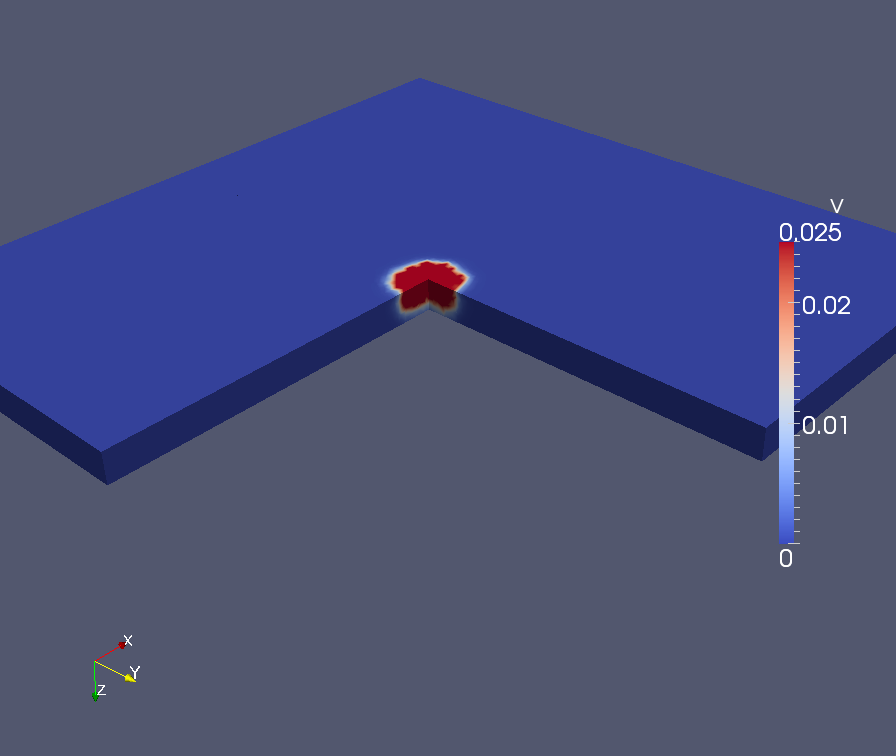
\includegraphics[width=\textwidth]{png/v-0001.png}
\caption{Начальное возмущение. На рисунке цветом изображены модули скоростей в
двух взаимно перпендикулярных срезах.}
\label{pic:multilayer_init}
\end{figure}
\begin{figure}[htp]
\centering
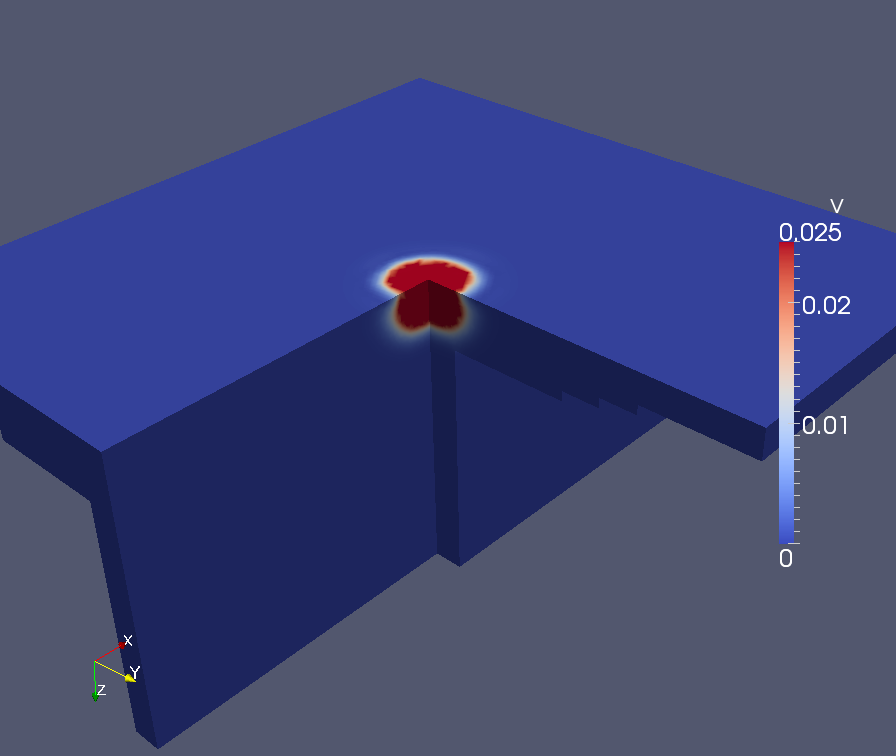
\includegraphics[width=\textwidth]{png/v-0003.png}
\caption{Отражение от первой границы. На рисунке цветом изображены модули скоростей в
двух взаимно перпендикулярных срезах.}
\label{pic:multilayer_b1}
\end{figure}
\begin{figure}[htp]
\centering
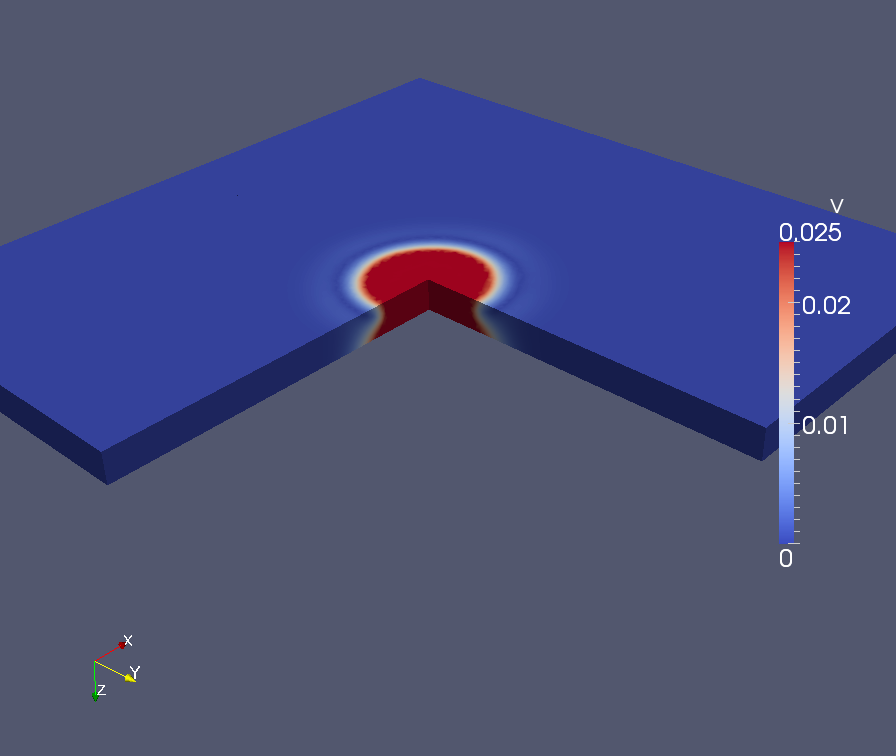
\includegraphics[width=\textwidth]{png/v-0007.png}
\caption{Отражение от второй границы. На рисунке цветом изображены модули скоростей в
двух взаимно перпендикулярных срезах.}
\label{pic:multilayer_b2}
\end{figure}
\begin{figure}[htp]
\centering
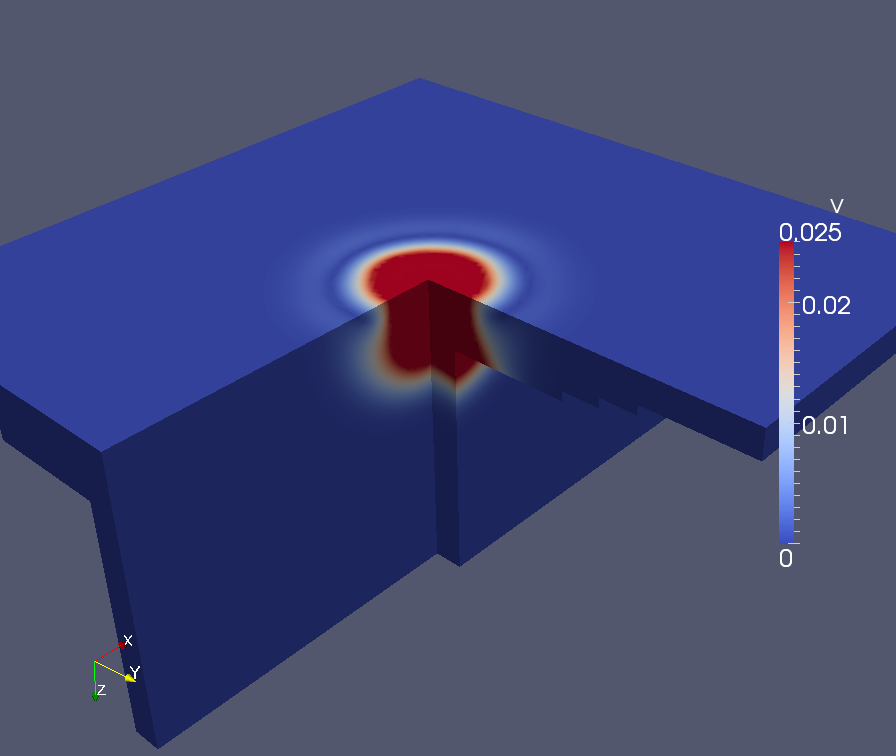
\includegraphics[width=\textwidth]{png/v-0009.png}
\caption{Отражение от третьей границы. На рисунке цветом изображены модули скоростей в
двух взаимно перпендикулярных срезах.}
\label{pic:multilayer_b3}
\end{figure}
\begin{figure}[htp]
\centering
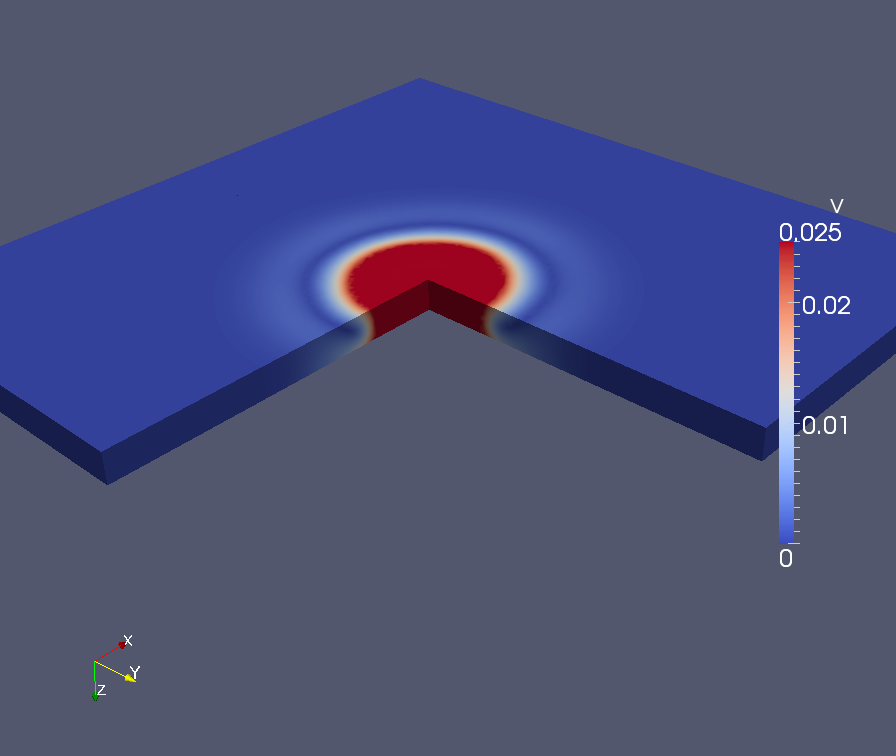
\includegraphics[width=\textwidth]{png/v-0013.png}
\caption{Формирование волны Рэлея. На рисунке цветом изображены модули скоростей
в срезе, перпендикулярном оси x, а стрелками обозначены поля скоростей.}
\label{pic:multilayer_Rayleigh_1}
\end{figure}
\begin{figure}[htp]
\centering
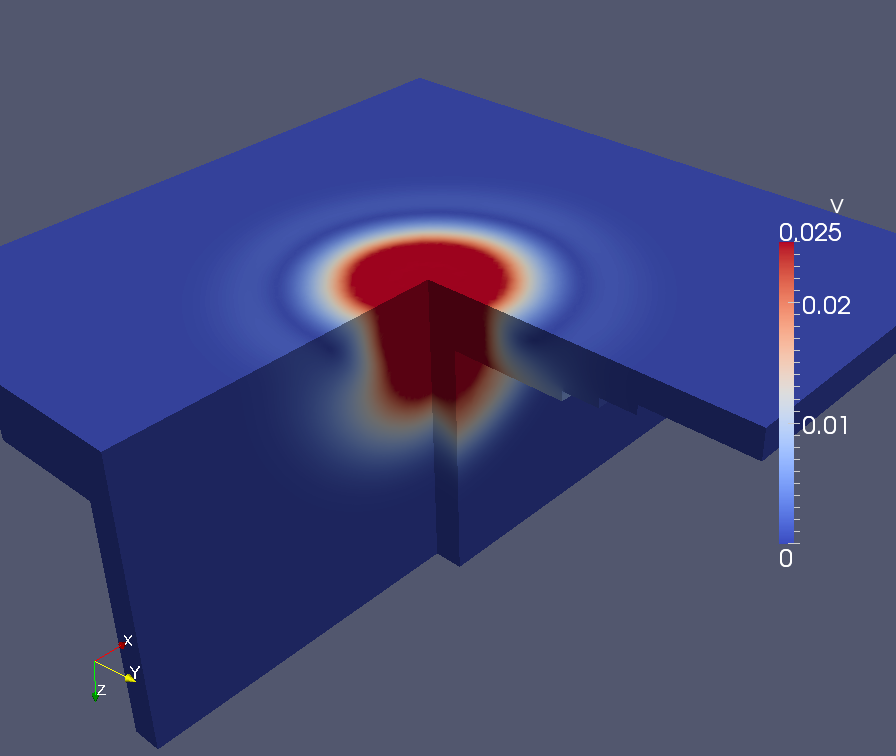
\includegraphics[width=\textwidth]{png/v-0016.png}
\caption{Распространение волны Рэлея. На рисунке цветом изображены модули скоростей
в срезе, перпендикулярном оси x, а стрелками обозначены поля скоростей.}
\label{pic:multilayer_Rayleigh_2}
\end{figure}
